\begin{figure}[htbp]
\centering
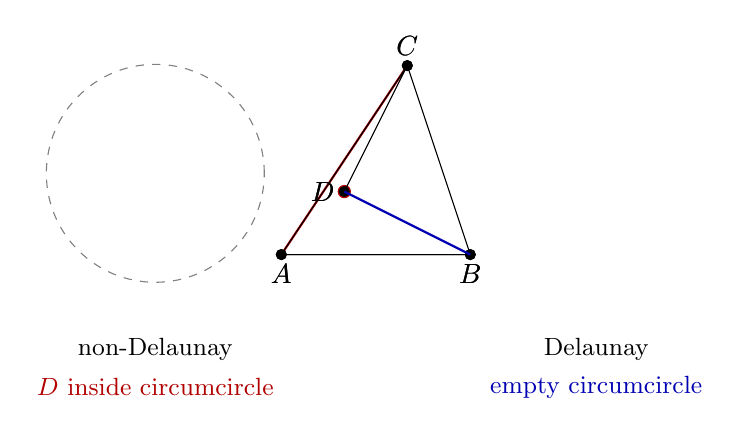
\begin{tikzpicture}[scale=0.8]
  \coordinate (A) at (0,0);
  \coordinate (B) at (3,0);
  \coordinate (C) at (2,3);
  \coordinate (D) at (1,1);
  \begin{scope}[xshift=-3.5cm]
    \fill (A) circle (2.5pt) node[below] {$A$};
    \fill (B) circle (2.5pt) node[below] {$B$};
    \fill (C) circle (2.5pt) node[above] {$C$};
    \fill (D) circle (2.5pt) node[left] {$D$};
    \draw (A)--(B)--(C)--cycle;
    \draw[red!70!black,thick] (A)--(C);
    \draw[gray,dashed] (1.5,1.29) circle (1.73);
    \fill[red!70!black] (D) circle (3pt);
    \node at (1.5,-1.5) {\small non-Delaunay};
    \node[red!70!black] at (1.5,-2.1) {\small $D$ inside circumcircle};
  \end{scope}
  \begin{scope}[xshift=3.5cm]
    \fill (A) circle (2.5pt) node[below] {$A$};
    \fill (B) circle (2.5pt) node[below] {$B$};
    \fill (C) circle (2.5pt) node[above] {$C$};
    \fill (D) circle (2.5pt) node[left] {$D$};
    \draw (A)--(B)--(D)--(C)--cycle;
    \draw[blue!70!black,thick] (B)--(D);
    \node at (1.5,-1.5) {\small Delaunay};
    \node[blue!70!black] at (1.5,-2.1) {\small empty circumcircle};
  \end{scope}
\end{tikzpicture}
\caption{Delaunay property: (left)~edge $AC$ is illegal because $D$ lies inside the circumcircle of $ABC$. (right)~Flipping to edge $BD$ satisfies the empty circumcircle property.}
\label{fig:delaunay_flip}
\end{figure}
